\chapter{Conception de Gatling}
\section{Le DSL}
\subsection{Analyse d'un test de charge}
Afin de créer un DSL utile et simple à utiliser par les futurs utilisateurs de Gatling, une analyse d'une simulation (ou test de charge) a été faite afin de repérer les éléments que contient un scénario.

\subsubsection{Définition d'un scénario}
Afin de définir un scénario d'utilisation, la personne qui l'écrit doit pouvoir spécifier :
\begin{itemize}
  \item Le nom du scénario
  \item Les requêtes faites par l'utilisateur, et pour chaque requête :
  \begin{itemize}
    \item Le type de la requête (HTTP pour l'instant)
	\item Le nom de la requête (pour facilement identifier la requête dans les statistiques)
    \item Le verbe HTTP utilisé (POST, PUT, GET ou DELETE)
    \item Les paramètres de la requête
    \item Le corps de la requête si possible
  \end{itemize}
  \item Les pauses qui simulent le temps de lecture de l'utilisateur
\end{itemize}

\subsubsection{Exécution d'une simulation}
Une fois les scénarios écrits, il faudra les exécuter, et le testeur doit pouvoir configurer cette exécution. Voici les éléments configurables :
\begin{itemize}
  \item Le nombre d'utilisateurs simultanés pour ce scénario
  \item La rampe de démarrage des utilisateurs. Ceci permet de simuler un arrivage progressif des utilisateurs sur le site par exemple
  \item Le démarrage du scénario. En effet, plusieurs scénarios peuvent être exécutés durant une simulation, on peut donc spécifier à quel moment de la simulation le scénario doit démarrer.
\end{itemize}

\subsection{Définition du DSL}
Les éléments que l'analyse a permis de découvrir représentent la base du DSL. Pour fournir aux testeurs un DSL plus efficace et qui les aide à écrire des scénarios complexes plus simplement, d'autres éléments ont été ajoutés. Pour chaque éléments, vous trouverez un exemple du DSL qui correspond. Le logiciel étant Open Source et destiné aux entreprises du monde entier, le DSL est en anglais.


\subsubsection{Déclaration d'une requête HTTP}

Le DSL permet de déclarer et configurer facilement des requêtes HTTP. Le code du listing \ref{declare_request} montre quelques unes des diverses possibilités offertes. 

\begin{lstlisting}[caption={Déclaration d'une requête HTTP},label={declare_request}]
// Faire une requete de type GET sur l'url http://google.fr
get("http://google.fr")

// Faire une requete de type GET sur 
// l'url http://google.fr?q=ma+recherche
get("http://google.fr") withQueryParam ("q", "ma+recherche")

// Faire une requete de type POST sur l'url http://monurl.com
// avec le corps : '{"mon_object": {"attribut": "valeur" }'
// et des headers specifiant le contenu : JSON
post("http://monurl.com")
   withBody """{ "mon_object" : { "attribut": "valeur" }"""
   asJSON

// Faire une requete de type PUT sur l'url http://monurl.com
// avec le parametre de formulaire 'name' = 'John'
put("http://monurl.com") withParam ("name", "John")
\end{lstlisting}

\subsubsection{Déclaration d'un scénario}

L'exemple suivant, montré dans le listing \ref{declare_scenario}, illustre la façon dont un scénario peut être créé via le DSL de Gatling. Un scénario basique permettant de tester une application web contient des requêtes de type HTTP, ainsi que des pauses permettant de simuler le temps de lecture de l'utilisateur.

\begin{lstlisting}[caption={Déclaration d'un scénario simple},label={declare_scenario}]
// Declarer un scenario nomme 'S1', constitue d'une requete 
// sur le site de Google, attendre 1 seconde puis executer 
// une requete de recherche.
scenario("S1")
  doHttpRequest("Accueil", get("http://google.fr"))
  pause(1)
  doHttpRequest("Recherche", get("http://google.fr") 
    withQueryParam ("q", "keyword")
\end{lstlisting}

\subsubsection{Déclaration d'une simulation}

La dernière étape, une fois le scénario écrit, consiste à le configurer pour l'exécuter. Le listing \ref{declare_all} montre de quelle façon est déclarée la configuration puis la demande d'exécution de la simulation.

\begin{lstlisting}[caption={Déclaration d'une simulation au complet},label={declare_all}]
// On declare un scenario
val stdUser = scenario("Standard") do...

// On cree une configuration pour ce scenario avec
// * 5 utilisateurs concurrents
// * 0 seconde de rampe
// * 0 seconde de delai au demarrage
val stdUserConf = 
  configureScenario(stdUser)
    withUsersNumber 5 
    withRamp 0
    startsAt 0
val execution = runSimulations(stdUserConf)
\end{lstlisting}

\subsection{Fonctionnalités supplémentaires du DSL}
Afin de simplifier l'écriture des scénarios et d'augmenter les possibilités du DSL, des fonctionnalités supplémentaires ont été ajoutées.

\subsubsection{Captures et assertions}
Afin de valider les requêtes, le testeur pourra utiliser des assertions sur la réponse HTTP, permettant de vérifier sont code, ainsi que la présence de certains headers ou des expressions dans le corps de la réponse. Cela permettra par exemple de valider une requête de login avant d'exécuter le reste du scénario. 

Les assertions sont basées sur les captures qui permettent de faire des recherches par expression régulière ou par XPath. Ces captures sont exécutées sur la réponse HTTP reçue par le moteur de simulation. Chacun de ces \em{processeur} est disponible indépendament de l'autre dans le DSL, le listing \ref{use_capture_and_assertion} montre comment ils sont utilisés.

\begin{lstlisting}[caption={Utilisation des captures et assertions},label={use_capture_and_assertion}]
scenario("S1")
  doHttpRequest(
    "Accueil",
    get("http://www.google.fr"),
    // On stocke "ou" dans "name"
    regexp("""Ab(.*)t""") in "name",
    // On verifie qu'on est bien sur google
    assertRegexp("""<img alt="(.*)" """, "Google")
  )
\end{lstlisting}

\subsubsection{Contexte}
Un contexte est présent pour chaque scénario, et est propre à un seul utilisateur simulé par ce scénario. La présence de ce contexte permet au testeur de faire passer des infos de requête en requêtes.

Le testeur pourra extraire des données des réponses HTTP afin de les stocker dans le contexte, cela se fera en utilisant des captures (ou des assertions), les valeurs seront ensuite accessibles dans le reste du scénario. Le listing \ref{use_context} montre l'utilisation du contexte dans le cadre d'un scenario simple.

\begin{lstlisting}[caption={Utilisation du contexte},label={use_context}]
scenario("S1")
  doHttpRequest(
    "Set Value",
    get("http://google.fr"),
    regexp("""<img alt="(.*)" """) in "pagename")
  pause(1)
  doHttpRequest(
  	"Use value",
  	get("http://google.fr") 
  	  withQueryParam ("q", FromContext("pagename")))
\end{lstlisting}

\subsubsection{Feeders (ou Seeders)}
La simulation d'un grand nombre d'utilisateurs peut nécessiter l'utilisation d'un aussi grand nombre de comptes différents sur l'application testée. Pour permettre l'utilisation d'un compte différent par utilisateur simulé, Gatling propose des Feeders\footnote{ou Seeders, le nom n'étant pas encore figé}. Ces éléments permettent d'utiliser une source de données telles qu'un fichiers de type CSV pour y récupérer des informations à utiliser dans le scénario. Le listing \ref{use_feeder} montre l'utilisation de ces Feeders dans le cadre d'un scénario simple.

\begin{lstlisting}[caption={Utilisation des Feeders},label={use_feeder}]
// Declaration du Feeder
userCredentials = 
  new CSVFeeder("user_cred", List("login", "password"))

scenario("S1")
  doHttpRequest(
    "Login",
    post("http://mywebsite.com/login")
      // Declaration du Feeder pour cette requete
      withFeeder userCredentials
      // Utilisation des parametres du feeder
      withParam "login"
      withParam "password"
\end{lstlisting}


\section{Architecture de Gatling}
\subsection{Entrées \& sorties}
Gatling, comme tout programme informatique, accepte des données en entrée et renvoie des données en sortie. Les entrées sont créées par l'utilisateur de l'outil, tandis que les sorties sont destinées à être interprétées par ce même utilisateur. La figure \ref{io} représente les entrées et sorties de Gatling, elles sont composées de :

\begin{itemize}
  \item Entrées
  \begin{itemize}
	\item \em{Scripts}. Les scripts sont des fichiers scala qui contiennent les scénarios et simulations que le testeur veut exécuter.
  	\item \em{Seeds}. Les seeds\footnote{Graines en français} contiennent les données qui seront utilisées par les feeders dans les scénarios.
  	\item \em{Bodies}. Les Bodies sont les corps envoyés avec les requêtes de type POST ou PUT.
  \end{itemize}
  \item Sorties
  \begin{itemize}
    \item \em{Rapports}. Les rapports générés au format HTML.
  \end{itemize}
\end{itemize}

\begin{figure}[h]
\begin{center}
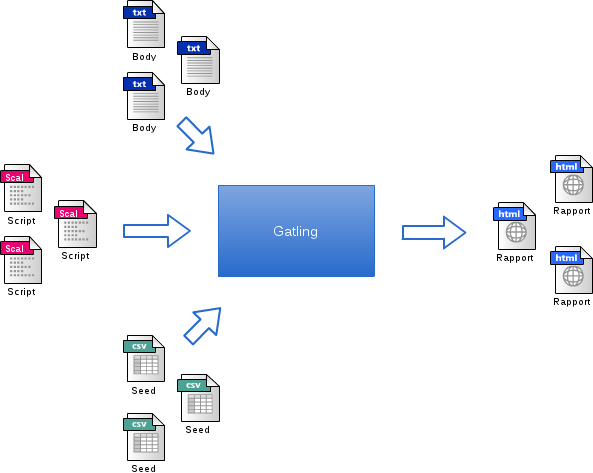
\includegraphics[width=400pt]{img/io.png}
\end{center}
\caption{Entrées et sorties de Gatling}
\label{io}
\end{figure}

\subsection{Structure des dossiers}
Afin de permettre à l'application comme à l'utilisateur de savoir où se trouvent les fichiers nécessaires à l'exécution d'une simulation, une structure de dossiers a été créée. Cette structure est représentée ci-après par la figure \ref{folders}.

\begin{figure}[h]
\begin{center}
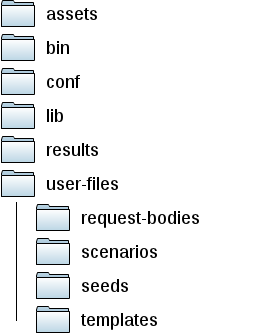
\includegraphics[width=175pt]{img/folders.png}
\end{center}
\caption{Structure de dossiers de Gatling}
\label{folders}
\end{figure}

Le dossier assets contient des fichiers utiles à la génération des rapports Les dossiers bin et lib contiennent les bibliothèques ainsi que l'exécutable qui permet de lancer Gatling. Le dossier conf contient le(s) fichier(s) de configuration de Gatling. Le dossier results contient les résultats de tests, rangés dans des dossiers portant comme nom la date et l'heure d'exécution du test.

Enfin, le dossier user-files contient les différents fichiers que l'utilisateur crée pour écrire ses scénarios. Le dossier scenarios contient les scripts écrits avec le DSL de Gatling. Le dossier request-bodies contient les corps de requête à être envoyés tels quels, alors que le dossier template contient des templates pouvant être complétés lors de l'exécution du scénario avant d'être envoyés. Le dossier seeds quant à lui contient les jeux de données utilisés par les feeders.

\subsection{Application modulaire}
Gatling est découpé en différents modules interagissant les uns avec les autres. Ce découpage permet de créer des APIs internes, ce qui facilite l'ajout de fonctionnalités similaires comme, par exemple, l'ajout du support d'un protocole autre que HTTP. La figure \ref{arch} montre les modules principaux nécessaire au test d'applications web standard et présents dans la première version de l'application :
\begin{itemize}
  \item Gatling App. C'est l'interface avec l'utilisateur de l'application, en l'occurence par la ligne de commande.
  \item Gatling Http. Ce module fournit les classes permettant de supporter le protocole HTTP.
  \item Gatling Statistics. Ce module fournit les classes permettant de générer les rapports.
  \item Gatling Core. Ce module contient toutes les fonctionnalités au coeur de l'application.
\end{itemize}

\begin{figure}[h]
\begin{center}
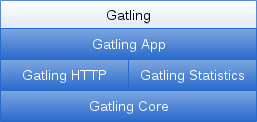
\includegraphics{img/arch.png}
\end{center}
\caption{Architecture de Gatling}
\label{arch}
\end{figure}

Dans la suite de ce chapitre, les différents modules seront présentés en détails.

\section{Gatling Core}
\subsection{}

\section{Gatling Http}

\section{Gatling Statistics}
Les statistiques sont générés selon le modèle de la figure \ref{stats_gen}. Lors de l'exécution du scénario, le moteur enregistre les résultats de chaque requête dans un fichier. Ce fichier est ensuite analysé par un extracteur de données qui récupère et formatte les données utiles à la génération d'un graphique. Ces données sont ensuite mise en forme par les presenters et enfin, un fichier de rapport est créé au format HTML grâce à l'utilisation de templates, comme vu section XXX.

\begin{figure}[h]
\begin{center}
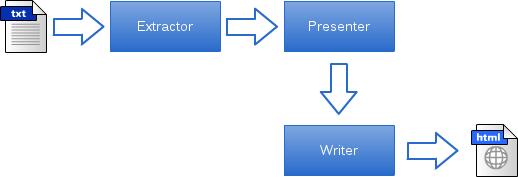
\includegraphics{img/stats_gen.png}
\end{center}
\caption{Génération de statistiques}
\label{stats_gen}
\end{figure}

\begin{figure}[h]
\begin{center}
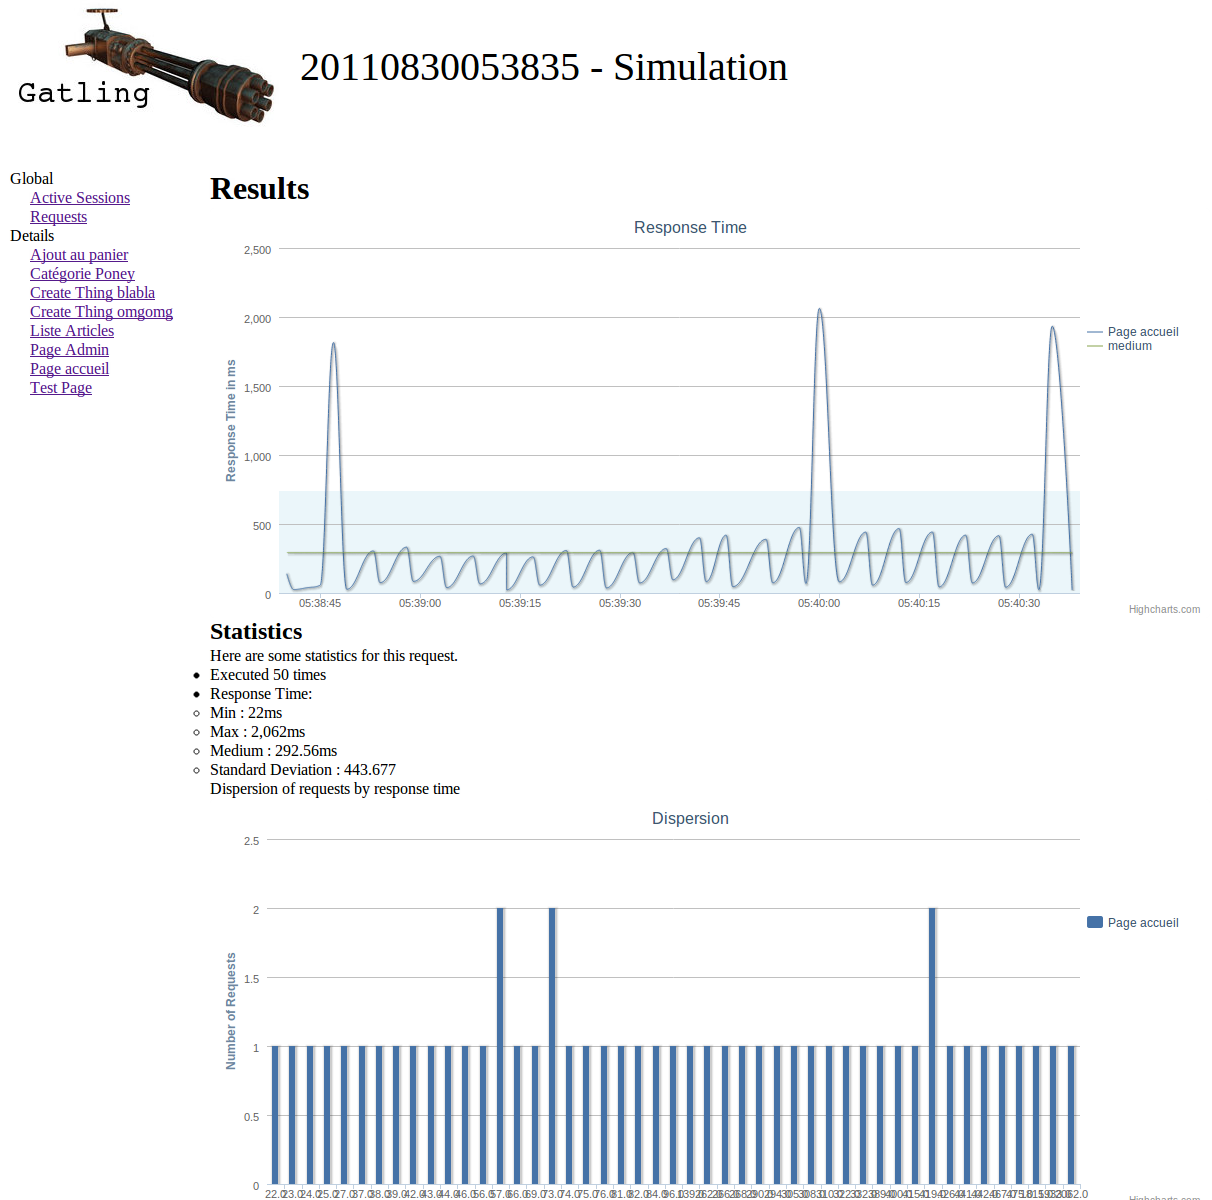
\includegraphics{img/stats_exp.png}
\end{center}
\caption{Exemple de statistiques générées}
\label{stats_gen}
\end{figure}